\subsection[Heap]{Heapsort}

\begin{frame}
	\frametitle{Tas (Heap)}
	Le tas est une structure de donnée qui a deux opérations:
	\begin{itemize}
		\item \texttt{push}: ajouter un élément au tas. $O(\log n)$.
		\item \texttt{pop}: retire l'élément le plus grand. $O(\log n)$.
	\end{itemize}
\end{frame}

\begin{frame}
\frametitle{Tri par tas (Heap sort)}
\framesubtitle{Idée}
\begin{itemize}
\item Mettre tout les élements dans un tas
\item Retirer les élements du tas, un à un
\end{itemize}
\end{frame}

\begin{frame}
\frametitle{Heapsort}
\begin{table}
\begin{tabular}{| c | c | c | c | c | c | c | c |}
\hline
8 & 6 & 7 & 4 & 5 & 3 & 2 & 1 \\ 
\hline
\end{tabular}
\end{table}

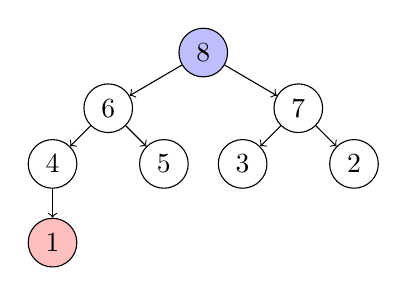
\begin{tikzpicture}[->,nodes={draw, circle}]
    \node (a8) [fill = blue!25] {8};
    \node (a6) [below left of = a8, xshift=-0.5cm] {6};
	\node (a7) [below right of = a8, xshift=0.5cm]{7};
	\node (a4) [below left of = a6]{4};
	\node (a5) [below right of = a6]{5};
	\node (a3) [below left of = a7]{3};
	\node (a2) [below right of = a7]{2};
	\node (a1) [below of = a4, fill = red!25]{1};
    
    \draw (a8) -> (a7);
    \draw (a8) -> (a6); 
    \draw (a6) -> (a4);
    \draw (a6) -> (a5);
    \draw (a7) -> (a3);
    \draw (a7) -> (a2);
    \draw (a4) -> (a1);
\end{tikzpicture}
\end{frame}

\begin{frame}
\frametitle{Heapsort}
\begin{table}
\begin{tabular}{| c | c | c | c | c | c | c | c |}
\hline
\cellcolor{red!25}1 & 6 & \cellcolor{green!25}7 & 4 & 5 & \cellcolor{green!25}3 & 2 & \cellcolor{black!25}8 \\  
\hline
\end{tabular}
\end{table}

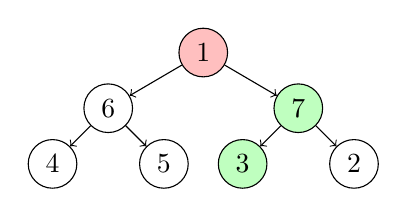
\begin{tikzpicture}[->,nodes={draw, circle}]
    \node (a1) [fill = red!25]{1};
    \node (a6) [below left of = a1, xshift=-0.5cm] {6};
	\node (a7) [below right of = a1, xshift=0.5cm, fill = green!25]{7};
	\node (a4) [below left of = a6]{4};
	\node (a5) [below right of = a6]{5};
	\node (a3) [below left of = a7, fill = green!25]{3};
	\node (a2) [below right of = a7]{2};
    
    \draw (a1) -> (a7);
    \draw (a1) -> (a6); 
    \draw (a6) -> (a4);
    \draw (a6) -> (a5);
    \draw (a7) -> (a3);
    \draw (a7) -> (a2);
\end{tikzpicture}
\end{frame}

\begin{frame}
\frametitle{Heapsort}
\begin{table}
\begin{tabular}{| c | c | c | c | c | c | c | c |}
\hline
\cellcolor{blue!25}7 & 6 & 3 & 4 & 5 & 1 & \cellcolor{red!25}2 & \cellcolor{black!25}8 \\  
\hline
\end{tabular}
\end{table}

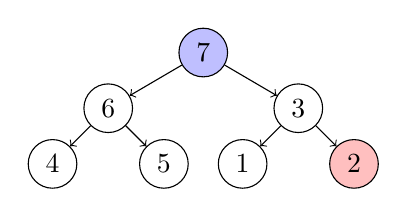
\begin{tikzpicture}[->,nodes={draw, circle}]
    \node (a7) [fill = blue!25]{7};
    \node (a6) [below left of = a7, xshift=-0.5cm] {6};
	\node (a3) [below right of = a7, xshift=0.5cm]{3};
	\node (a4) [below left of = a6]{4};
	\node (a5) [below right of = a6]{5};
	\node (a1) [below left of = a3]{1};
	\node (a2) [below right of = a3, fill = red!25]{2};
    
    \draw (a7) -> (a3);
    \draw (a7) -> (a6); 
    \draw (a6) -> (a4);
    \draw (a6) -> (a5);
    \draw (a3) -> (a1);
    \draw (a3) -> (a2);
\end{tikzpicture}
\end{frame}

\begin{frame}
\frametitle{Heapsort}
\begin{table}
\begin{tabular}{| c | c | c | c | c | c | c | c |}
\hline
\cellcolor{red!25}2 & \cellcolor{green!25}6 & 3 & 4 & \cellcolor{green!25}5 & 1 & \cellcolor{black!25}7 & \cellcolor{black!25}8 \\  
\hline
\end{tabular}
\end{table}

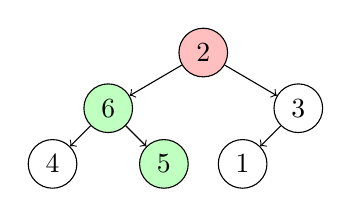
\begin{tikzpicture}[->,nodes={draw, circle}]
    \node (a2) [fill = red!25]{2};
    \node (a6) [below left of = a2, xshift=-0.5cm, fill = green!25] {6};
	\node (a3) [below right of = a2, xshift=0.5cm]{3};
	\node (a4) [below left of = a6]{4};
	\node (a5) [below right of = a6, fill = green!25]{5};
	\node (a1) [below left of = a3]{1};
    
    \draw (a2) -> (a6);
    \draw (a2) -> (a3); 
    \draw (a6) -> (a4);
    \draw (a6) -> (a5);
    \draw (a3) -> (a1);
\end{tikzpicture}
\end{frame}

\begin{frame}
\frametitle{Heapsort}
\begin{table}
\begin{tabular}{| c | c | c | c | c | c | c | c |}
\hline
\cellcolor{blue!25}6 & 5 & 3 & 4 & 2 & \cellcolor{red!25}1 & \cellcolor{black!25}7 & \cellcolor{black!25}8 \\  
\hline
\end{tabular}
\end{table}

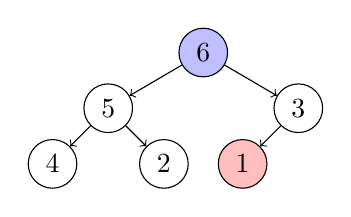
\begin{tikzpicture}[->,nodes={draw, circle}]
    \node (a6) [fill = blue!25]{6};
    \node (a5) [below left of = a6, xshift=-0.5cm] {5};
	\node (a3) [below right of = a6, xshift=0.5cm]{3};
	\node (a4) [below left of = a5]{4};
	\node (a2) [below right of = a5]{2};
	\node (a1) [below left of = a3, fill = red!25]{1};
    
    \draw (a6) -> (a5);
    \draw (a6) -> (a3); 
    \draw (a5) -> (a4);
    \draw (a5) -> (a2);
    \draw (a3) -> (a1);
\end{tikzpicture}
\end{frame}

\begin{frame}
\frametitle{Heapsort}
\begin{table}
\begin{tabular}{| c | c | c | c | c | c | c | c |}
\hline
\cellcolor{red!25}1 & \cellcolor{green!25}5 & 3 & \cellcolor{green!25}4 & 2 & \cellcolor{black!25}6 & \cellcolor{black!25}7 & \cellcolor{black!25}8 \\  
\hline
\end{tabular}
\end{table}

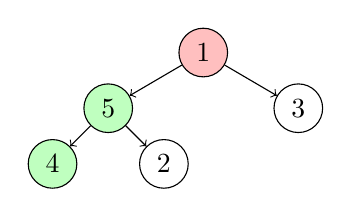
\begin{tikzpicture}[->,nodes={draw, circle}]
    \node (a1) [fill = red!25]{1};
    \node (a5) [below left of = a1, xshift=-0.5cm, fill = green!25] {5};
	\node (a3) [below right of = a1, xshift=0.5cm]{3};
	\node (a4) [below left of = a5, fill = green!25]{4};
	\node (a2) [below right of = a5]{2};
    
    \draw (a1) -> (a5);
    \draw (a1) -> (a3); 
    \draw (a5) -> (a4);
    \draw (a5) -> (a2);
\end{tikzpicture}
\end{frame}

\begin{frame}
\frametitle{Heapsort}
\begin{table}
\begin{tabular}{| c | c | c | c | c | c | c | c |}
\hline
\cellcolor{blue!25}5 & 4 & 3 & 1 & \cellcolor{red!25}2 & \cellcolor{black!25}6 & \cellcolor{black!25}7 & \cellcolor{black!25}8 \\  
\hline
\end{tabular}
\end{table}

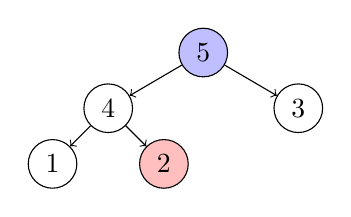
\begin{tikzpicture}[->,nodes={draw, circle}]
    \node (a5) [fill = blue!25]{5};
    \node (a4) [below left of = a5, xshift=-0.5cm] {4};
	\node (a3) [below right of = a5, xshift=0.5cm] {3};
	\node (a1) [below left of = a4] {1};
	\node (a2) [below right of = a4, fill = red!25] {2};
    
    \draw (a5) -> (a4);
    \draw (a5) -> (a3); 
    \draw (a4) -> (a1);
    \draw (a4) -> (a2);
\end{tikzpicture}
\end{frame}

\begin{frame}
\frametitle{Heapsort}
\begin{table}
\begin{tabular}{| c | c | c | c | c | c | c | c |}
\hline
\cellcolor{red!25}2 & \cellcolor{green!25}4 & 3 & 1 & \cellcolor{black!25}5 & \cellcolor{black!25}6 & \cellcolor{black!25}7 & \cellcolor{black!25}8 \\  
\hline
\end{tabular}
\end{table}

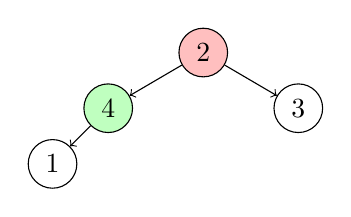
\begin{tikzpicture}[->,nodes={draw, circle}]
    \node (a2) [fill = red!25] {2};
    \node (a4) [below left of = a2, xshift=-0.5cm, fill = green!25] {4};
	\node (a3) [below right of = a2, xshift=0.5cm] {3};
	\node (a1) [below left of = a4] {1};
    
    \draw (a2) -> (a4);
    \draw (a2) -> (a3); 
    \draw (a4) -> (a1);
\end{tikzpicture}
\end{frame}

\begin{frame}
\frametitle{Heapsort}
\begin{table}
\begin{tabular}{| c | c | c | c | c | c | c | c |}
\hline
\cellcolor{blue!25}4 & 2 & 3 & \cellcolor{red!25}1 & \cellcolor{black!25}5 & \cellcolor{black!25}6 & \cellcolor{black!25}7 & \cellcolor{black!25}8 \\  
\hline
\end{tabular}
\end{table}

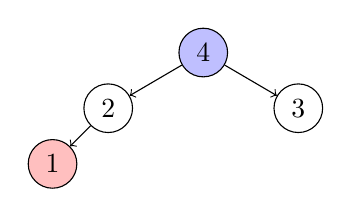
\begin{tikzpicture}[->,nodes={draw, circle}]
    \node (a4) [fill = blue!25]{4};
    \node (a2) [below left of = a4, xshift=-0.5cm] {2};
	\node (a3) [below right of = a4, xshift=0.5cm] {3};
	\node (a1) [below left of = a2, fill = red!25] {1};
    
    \draw (a4) -> (a2);
    \draw (a4) -> (a3); 
    \draw (a2) -> (a1);
\end{tikzpicture}
\end{frame}

\begin{frame}
\frametitle{Heapsort}
\begin{table}
\begin{tabular}{| c | c | c | c | c | c | c | c |}
\hline
\cellcolor{red!25}1 & 2 & \cellcolor{green!25}3 & \cellcolor{black!25}4 & \cellcolor{black!25}5 & \cellcolor{black!25}6 & \cellcolor{black!25}7 & \cellcolor{black!25}8 \\  
\hline
\end{tabular}
\end{table}

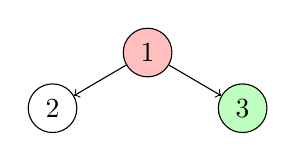
\begin{tikzpicture}[->,nodes={draw, circle}]
    \node (a1) [fill = red!25]{1};
    \node (a2) [below left of = a1, xshift=-0.5cm] {2};
	\node (a3) [below right of = a1, xshift=0.5cm, fill = green!25] {3};
    
    \draw (a1) -> (a2);
    \draw (a1) -> (a3); 
\end{tikzpicture}
\end{frame}

\begin{frame}
\frametitle{Heapsort}
\begin{table}
\begin{tabular}{| c | c | c | c | c | c | c | c |}
\hline
\cellcolor{blue!25}3 & 2 & \cellcolor{red!25}1 & \cellcolor{black!25}4 & \cellcolor{black!25}5 & \cellcolor{black!25}6 & \cellcolor{black!25}7 & \cellcolor{black!25}8 \\  
\hline
\end{tabular}
\end{table}

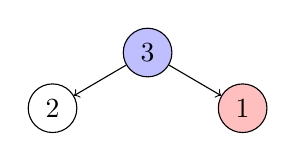
\begin{tikzpicture}[->,nodes={draw, circle}]
    \node (a3) [fill = blue!25]{3};
    \node (a2) [below left of = a3, xshift=-0.5cm] {2};
	\node (a1) [below right of = a3, xshift=0.5cm, fill = red!25] {1};
    
    \draw (a3) -> (a2);
    \draw (a3) -> (a1); 
\end{tikzpicture}
\end{frame}

\begin{frame}
\frametitle{Heapsort}
\begin{table}
\begin{tabular}{| c | c | c | c | c | c | c | c |}
\hline
\cellcolor{red!25}1 & \cellcolor{green!25}2 & \cellcolor{black!25}3 & \cellcolor{black!25}4 & \cellcolor{black!25}5 & \cellcolor{black!25}6 & \cellcolor{black!25}7 & \cellcolor{black!25}8 \\  
\hline
\end{tabular}
\end{table}

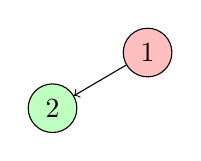
\begin{tikzpicture}[->,nodes={draw, circle}]
    \node (a1) [fill = red!25]{1};
    \node (a2) [below left of = a1, xshift=-0.5cm, fill = green!25] {2};
    
    \draw (a1) -> (a2); 
\end{tikzpicture}
\end{frame}

\begin{frame}
\frametitle{Heapsort}
\begin{table}
\begin{tabular}{| c | c | c | c | c | c | c | c |}
\hline
\cellcolor{blue!25}2 & \cellcolor{red!25}1 & \cellcolor{black!25}3 & \cellcolor{black!25}4 & \cellcolor{black!25}5 & \cellcolor{black!25}6 & \cellcolor{black!25}7 & \cellcolor{black!25}8 \\  
\hline
\end{tabular}
\end{table}

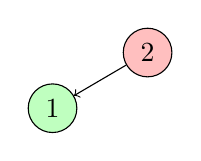
\begin{tikzpicture}[->,nodes={draw, circle}]
    \node (a2) [fill = red!25]{2};
    \node (a1) [below left of = a2, xshift=-0.5cm, fill = green!25] {1};
    
    \draw (a2) -> (a1); 
\end{tikzpicture}
\end{frame}

\begin{frame}
\frametitle{Heapsort}
\begin{table}
\begin{tabular}{| c | c | c | c | c | c | c | c |}
\hline
\cellcolor{red!25}1 & \cellcolor{black!25}2 & \cellcolor{black!25}3 & \cellcolor{black!25}4 & \cellcolor{black!25}5 & \cellcolor{black!25}6 & \cellcolor{black!25}7 & \cellcolor{black!25}8 \\  
\hline
\end{tabular}
\end{table}

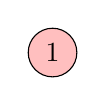
\begin{tikzpicture}[->,nodes={draw, circle}]
    \node (a1) [fill = red!25]{1};
    
\end{tikzpicture}
\end{frame}

\begin{frame}
\frametitle{Heapsort}
\begin{table}
\begin{tabular}{| c | c | c | c | c | c | c | c |}
\hline
\cellcolor{black!25}1 & \cellcolor{black!25}2 & \cellcolor{black!25}3 & \cellcolor{black!25}4 & \cellcolor{black!25}5 & \cellcolor{black!25}6 & \cellcolor{black!25}7 & \cellcolor{black!25}8 \\  
\hline
\end{tabular}
\end{table}
\end{frame}

\begin{frame}
\frametitle{Heapsort}
\framesubtitle{Complexité}
\begin{table}
\begin{tabular}{| c | c | c | c |}
\hline
Moyenne & Meilleure & Pire & Mémoire\\ 
\hline
O(n log(n)) & O(n log(n)) & O(n log(n)) & O(1)\\
\hline
\end{tabular}
\end{table}
\end{frame}